
\section{Our Datasets}

Before we begin testing we summarise what data we have so far and if we require any more. 

Each month has 2138 days of rainfall data. Due to unforseen issues with the Baum-Welch algorithm we used only 1000 of this for training. The remaining 1138 has been left aside for out of sample testing. If our simulations fit this dataset, it is a strong indication of success, as fitting the training set could just mean the model has fit the given data and not the generalised case. Thus we have two sets of recorded data; the training, of size 1000, and the test of size 1138.

When we first created our HMM in chapter 8 **ref** we also generated a simulation of size 1000 days. We will use this simulation for our testing now. From our parameter estimates in chapter 9 **ref** we generated simulations of size 1000 using "generator", which can be found in the "Model Generator" folder. 

Therefore we now have four sets of data two recorded, training and test,  and two simulated, HMM only and our Generalised HMM model.

\section{Results}

We carry out our testing in $"KS_tests.R"$.




\subsection{CDFs}

\begin{figure}
    \begin{subfigure}{.3\textwidth}
      \centering
      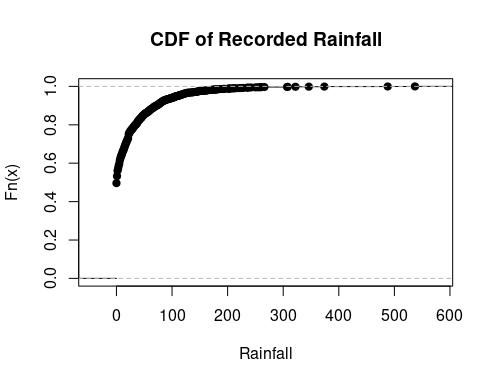
\includegraphics[width=\linewidth]{CDF/recorded.png}
      \caption{}
      \label{CDF:data}
    \end{subfigure}
    \begin{subfigure}{.3\textwidth}
      \centering
      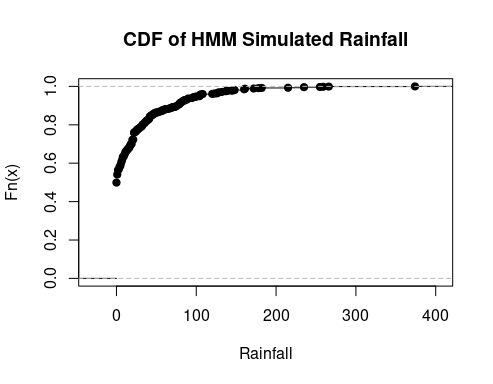
\includegraphics[width=\linewidth]{CDF/HMM.png}
      \caption{}
      \label{CDF:simhmm}
    \end{subfigure}
    \begin{subfigure}{.3\textwidth}
      \centering
      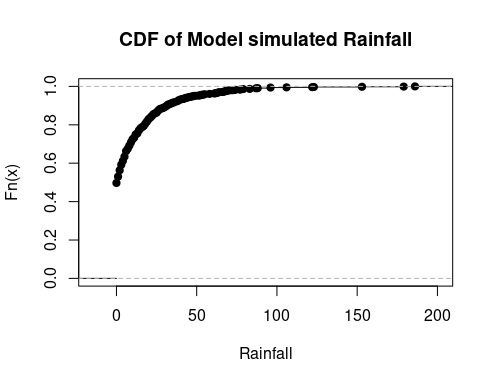
\includegraphics[width=\linewidth]{CDF/model.png}
      \caption{}
      \label{CDF:model}
    \end{subfigure}
    \caption{}
    \label{CDF}
\end{figure}

We begin by comparing the eprical cumulative distribution functions of each. We plot training and test data togther. From Figure~\ref{CDF} we can instantly see that neither the HMM only or our generalised model simulate any extreme values observed in the recorded data. However, the shape of the graphs seem similar as well as the rate of increase.


\subsection{Kologmorov-smirnof Tests}

To further test we apply the Kologmorov-Smirnof (KS) test for two samples **ref**. We apply this to both of our models against both training and test data. Our hyptohesis are given as follows:

\begin{itemize}
    \item $H_0$: The two samples are from the same distribution
    \item $H_1$: The two samples are not from the same distribution.
\end{itemize}

We will use a 5\% significance level for testing. Thus if the p-value is smaller than 0.05 we will reject the null hyptohesis.We record all four p-values for each month in the table given below.

\begin{center}
    \begin{tabular}{c c c c c}
              &  Train & Train     & Test &  Test \\	
        Month &	HMM	   & Gen Model & HMM  &	 Gen Model\\
        0	    &   0.8593	&   4.939$E^{-05}$	&   0.7899	    &       4.60$E^{-08}$   \\
        1	    &   0.9969	&   0.002038	&       0.105	    &       5.46$E^{-06}$   \\
        2	    &   1	    &   2.13$E^{-05}$	&   0.1118	    &       7.65$E^{-07}$   \\
        3	    &   1	    &   1.79$E^{-06}$	&   0.02163	    &       1.11$E^{-07}$   \\
        4	    &   0.4324	&   1.38$E^{-05}$	&   0.0009582	&       7.98$E^{-08}$   \\
        5	    &   1	    &   0.006202	&       0.2979	    &       0.0004948  \\
        6	    &   1	    &   1.11$E^{-05}$	&   0.1809	    &       8.53$E^{-08}$   \\
        7	    &   1	    &   2.13$E^{-05}$	&   0.03555	    &       4.53$E^{-05}$   \\
        8	    &   0.9999	&   0.0001108	&       0.07192	    &       0.001033   \\
        9	    &   0.9969	&   6.06$E^{-05}$	&   5.22$E^{-07}$	&   1.22$E^{-07}$   \\
        10	    &   0.8879	&   0.0008667	&       0.1914	    &       9.07$E^{-05}$   \\
        11	    &   0.9999	&   6.06$E^{-05}$	&   0.265	    &       2.15$E^{-06}$   

    \end{tabular}
\end{center}


It is clear to see that for all months, the KS test produces non-rejections. Thus one can assume the HMM describes the training data. For the test data we can see that for 4 out of 12 months we rejected the null hyptohesis. To find the justifications for why this is the case further testing is required. Initial thoughts include: maybe the training data was more similiar to the test for the 8 that did not reject or maybe the optima found through baum-welch was not infact a suitable optima. 

For our generaliseed model we rejected the null hypothesis every time when tested against both training and test sets. This suggests the model is not describing the rainfall data well. 